% !TeX root = ../main.tex

\section{Prozessablauf im Detail}

\begin{frame}{Prozessablauf im Detail}
    \begin{itemize}
        \item drei Phasen
        \begin{enumerate}
            \item Erster Zugriff auf SP und IdP
            \item Session Initialisierung und Authentifizierungsanfrage
            \item Authentifizierung, Autorisierung und Ressourcenzugriff~\cite{switchExpertDemoSWITCHaai2024a, shibbolethFlowsAndConfigShibbolethConcepts2019}
        \end{enumerate}
        \item Erklärung der einzelnen Phasen ...
        \item BPMN
    \end{itemize}
\end{frame}


\begin{frame}{Phase 1: Erster Zugriff}
    \begin{figure}
        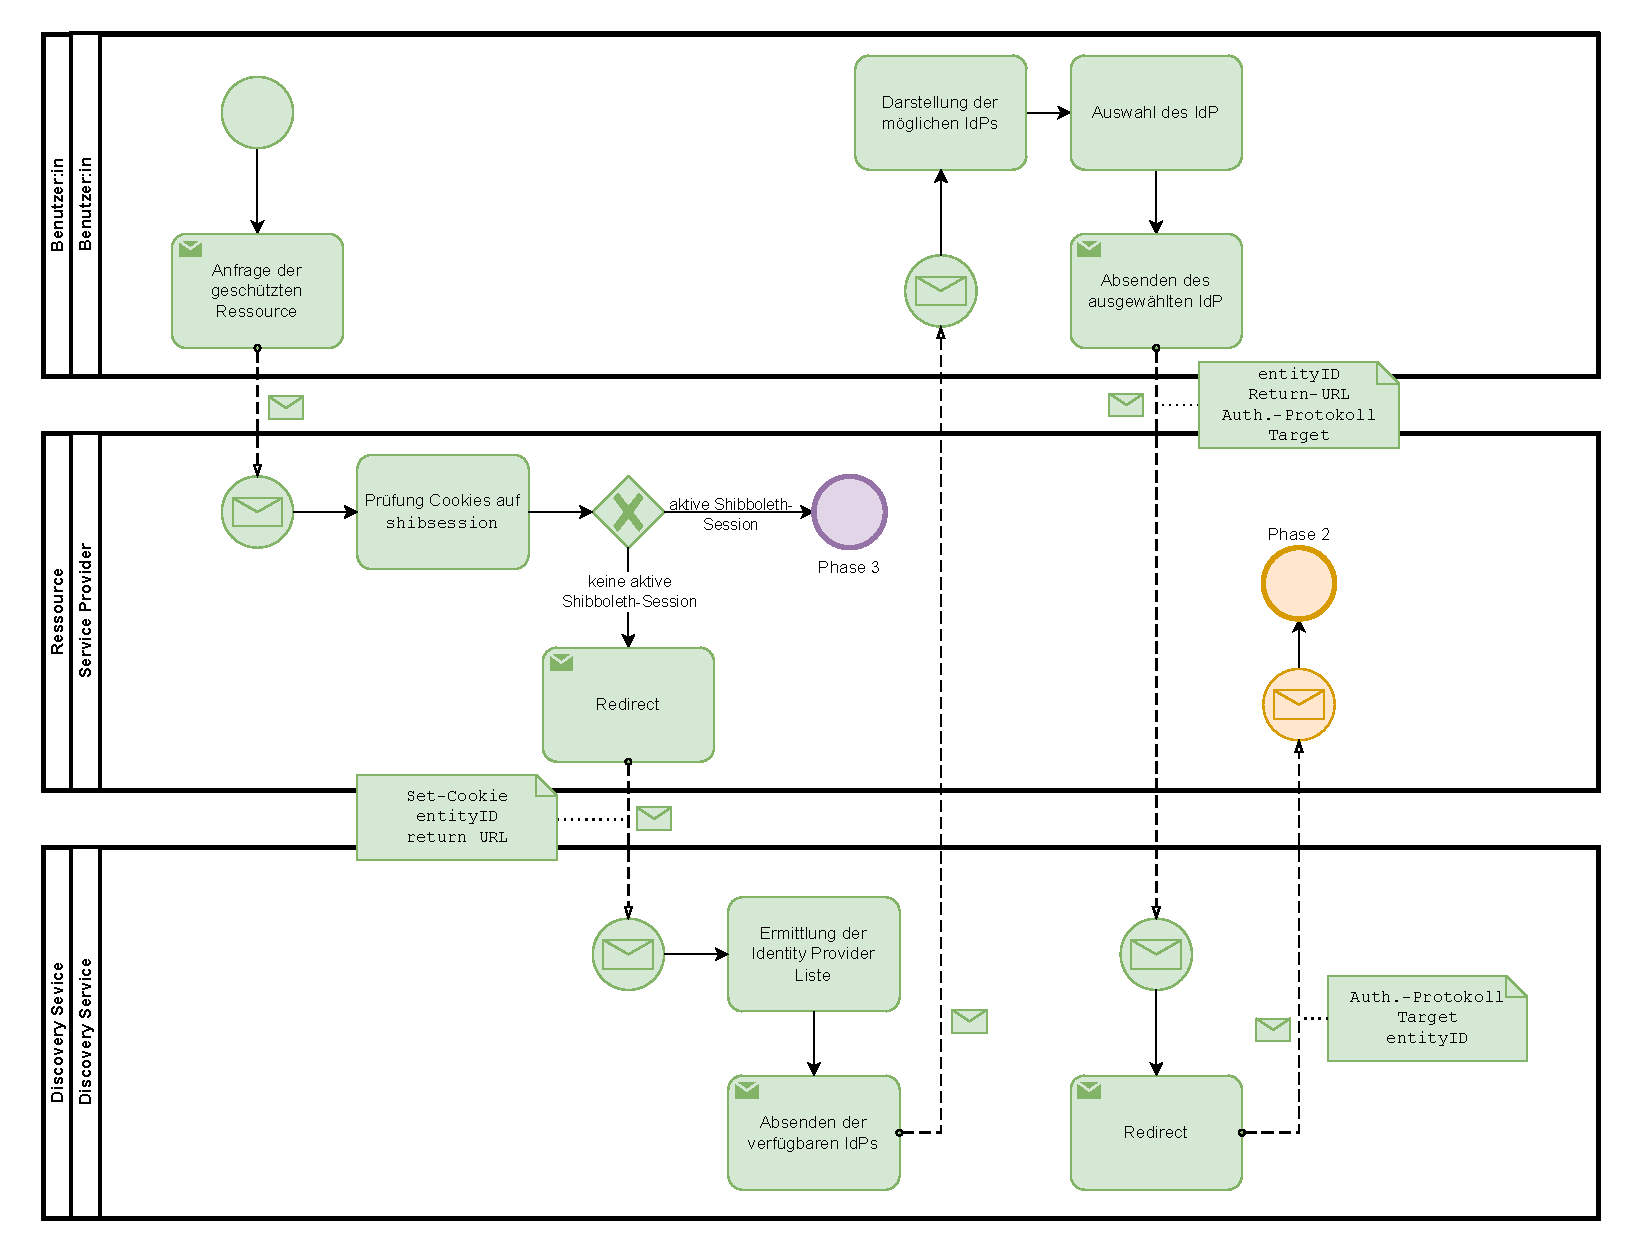
\includegraphics[height=0.7\paperheight]{../assets/bis_bpmn_phase_1.drawio.pdf}
        \caption{Phase 1 im Shibboleth-Prozess~\cite[vgl.][]{switchExpertDemoSWITCHaai2024a}}
    \end{figure}
\end{frame}


\begin{frame}{Phase 2: Session Initialisierung \& Authentifizierungsanfrage}
    \begin{figure}
        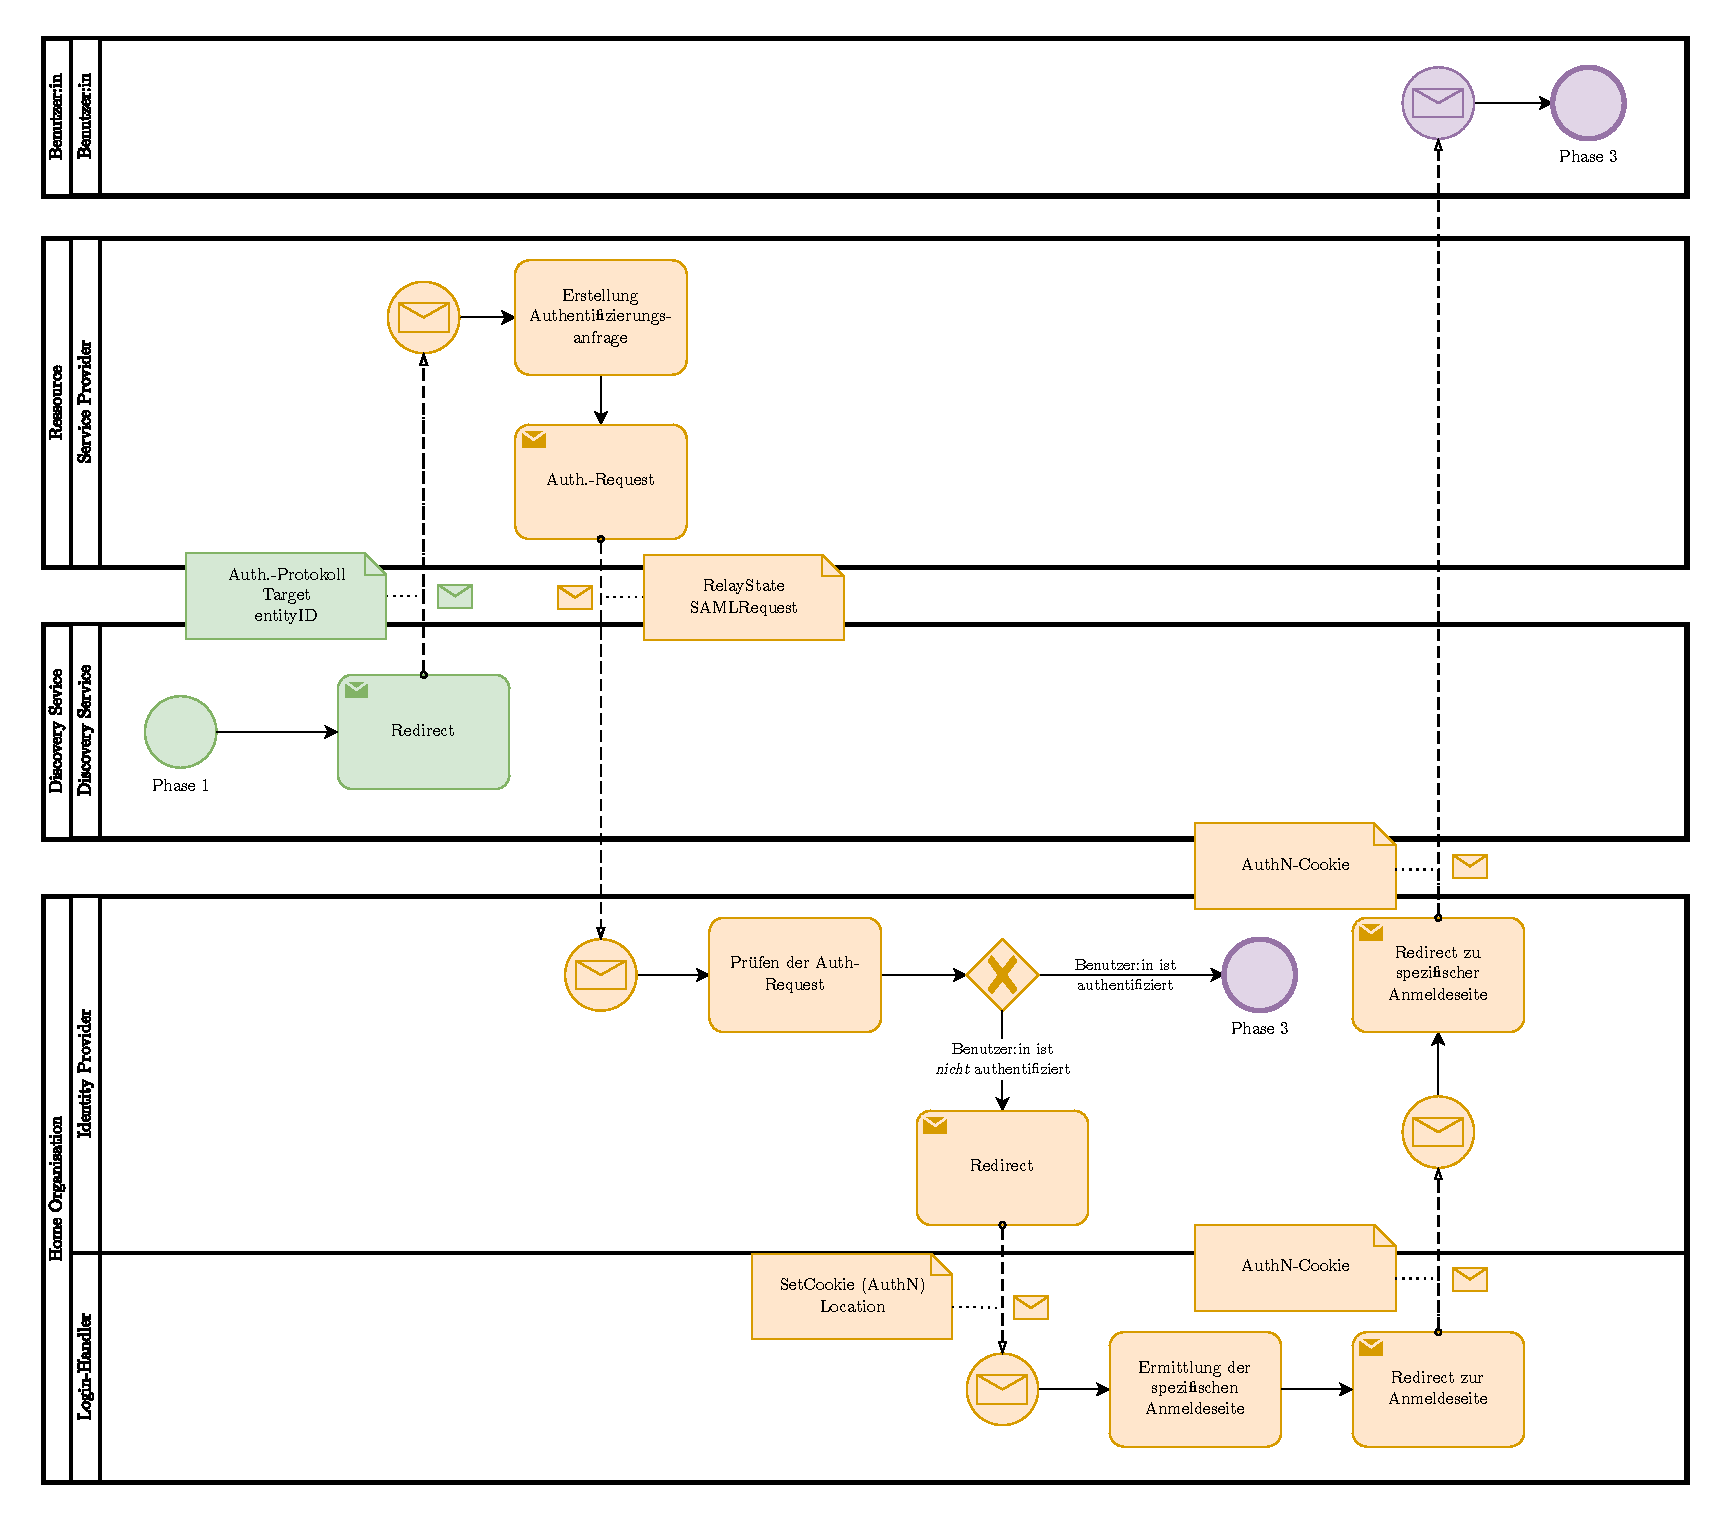
\includegraphics[height=0.7\paperheight]{../assets/bis_bpmn_phase_2.drawio.pdf}
        \caption{Phase 2 im Shibboleth-Prozess~\cite[vgl.][]{switchExpertDemoSWITCHaai2024a}}
    \end{figure}
\end{frame}


\begin{frame}{Phase 3: Authentifizierung, Autorisierung \& Ressourcenzugriff}
    \begin{figure}
        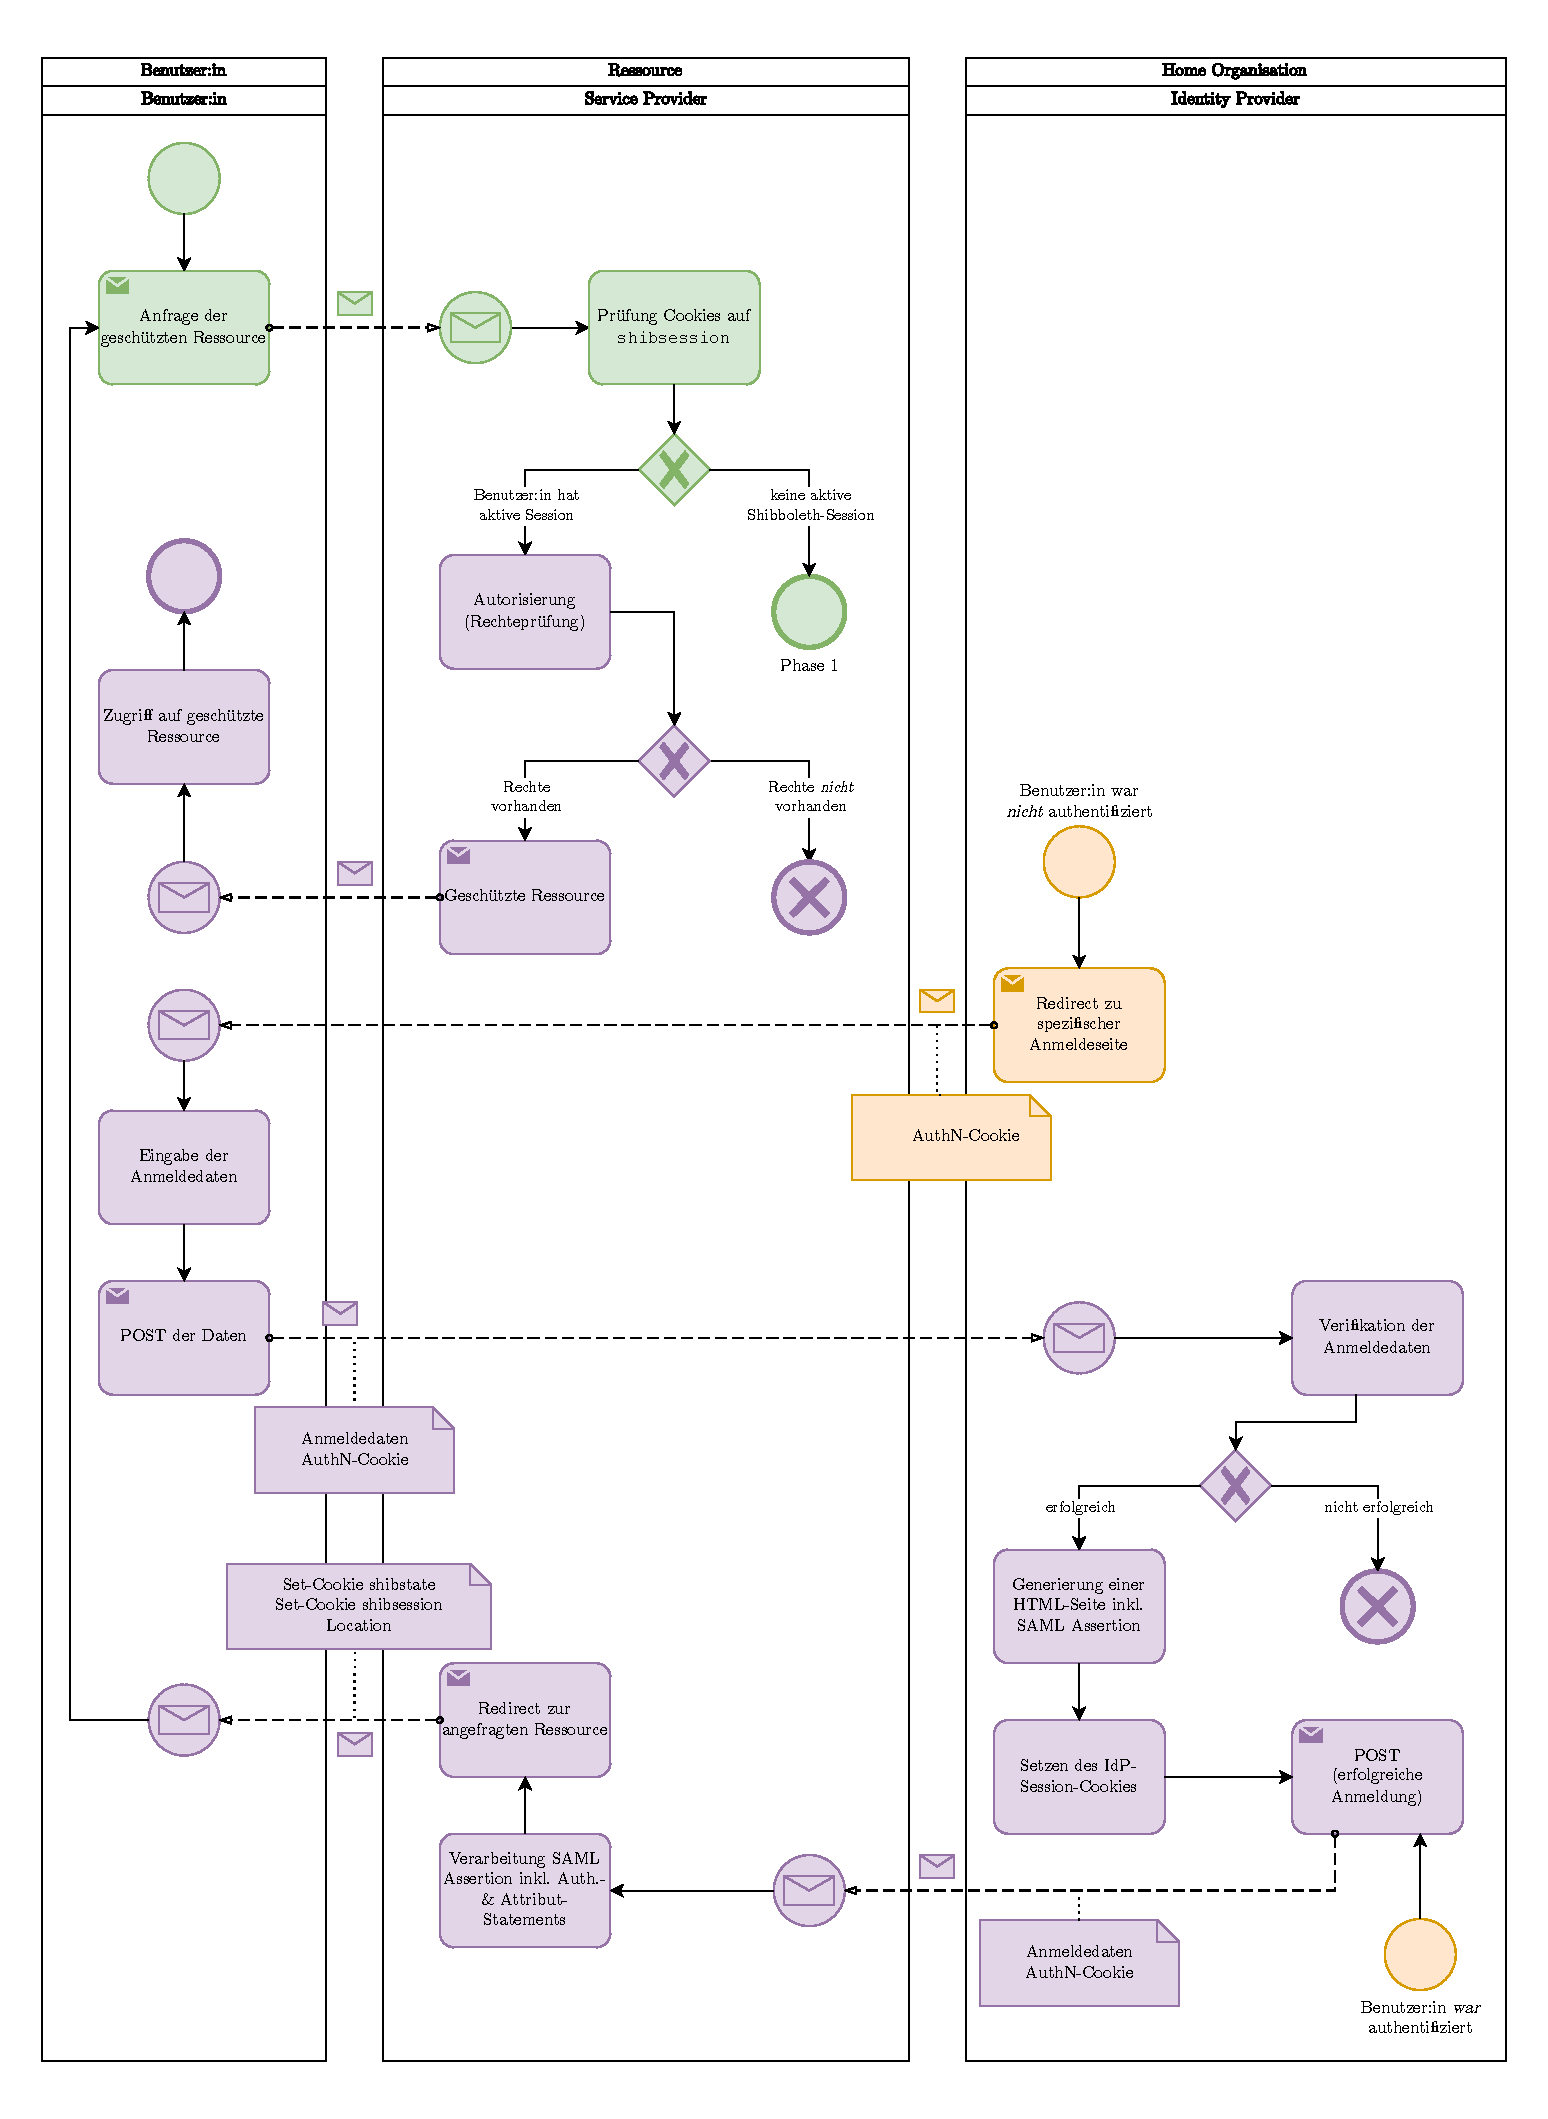
\includegraphics[height=0.7\paperheight]{../assets/bis_bpmn_phase_3.drawio.pdf}
        \caption{Phase 3 im Shibboleth-Prozess~\cite[vgl.][]{switchExpertDemoSWITCHaai2024a}}
    \end{figure}
\end{frame}
